% Template for PLoS
% Version 1.0 January 2009
%
% To compile to pdf, run:
% latex plos.template
% bibtex plos.template
% latex plos.template
% latex plos.template
% dvipdf plos.template

\documentclass[10pt,draft]{article}

% amsmath package, useful for mathematical formulas
\usepackage{amsmath}
% amssymb package, useful for mathematical symbols
\usepackage{amssymb}

% graphicx package, useful for including eps and pdf graphics
% include graphics with the command \includegraphics
\usepackage{graphicx}

% cite package, to clean up citations in the main text. Do not remove.
\usepackage{cite}

\usepackage{color} 

% Use doublespacing - comment out for single spacing
%\usepackage{setspace} 
%\doublespacing


% Text layout
\topmargin 0.0cm
\oddsidemargin 0.5cm
\evensidemargin 0.5cm
\textwidth 16cm 
\textheight 21cm

% Bold the 'Figure #' in the caption and separate it with a period
% Captions will be left justified
\usepackage[labelfont=bf,labelsep=period,justification=raggedright]{caption}

% Use the PLoS provided bibtex style
\bibliographystyle{plos2009}

% Remove brackets from numbering in List of References
\makeatletter
\renewcommand{\@biblabel}[1]{\quad#1.}
\makeatother


% Leave date blank
\date{}

\pagestyle{myheadings}
%% ** EDIT HERE **


%% ** EDIT HERE **
%% PLEASE INCLUDE ALL MACROS BELOW

%% END MACROS SECTION

\begin{document}

% Title must be 150 characters or less
\begin{flushleft}
{\Large
\textbf{Digital Normalization of Short Shotgun Sequences Facilitates
{\em de novo} Sequence Assembly}
}
% Insert Author names, affiliations and corresponding author email.
\\
C. Titus Brown$^{1,\ast}$, 
Adina Howe$^{2}$,
Qingpeng Zhang$^{3}$,
Alexis B. Pyrkosz$^{4}$,
Timothy H. Brom$^{3}$
\\
\bf{1} Departments of Computer Science and Engineering/Microbiology and Molecular Genetics, Michigan State University, East Lansing, MI, USA
\\
\bf{2} Departments of Microbiology and Molecular Genetics/Crop and Soil Sciences, Michigan State University, East Lansing, MI, USA
\\
\bf{3} Department of Computer Science and Engineering, Michigan State University, East Lansing, MI, USA
\\
{\bf{4} USDA Avian Disease and Oncology Laboratory, East Lansing, MI, USA}
\\
$\ast$ E-mail: Corresponding ctb@msu.edu
\end{flushleft}

% Please keep the abstract between 250 and 300 words
\section*{Abstract}

{\bf Background:} Deep shotgun sequencing and analysis of genomes,
transcriptomes, amplified single-cell genomes, and metagenomes enable
the sensitive investigation of a wide range of biological
phenomena. However, it is increasingly difficult to deal with the volume of data
emerging from deep short-read sequencers, in part because of random
and systematic sampling variation as well as many sequencing errors.
These challenges have led to the development of entire new classes of
short-read mapping tools such as Bowtie and BWA, as well as new de
novo assemblers such as ABySS, Velvet, SOAPdenovo, ALL-PATHS, and SGA.
Even newer assembly strategies for dealing with transcriptomes,
single-cell genomes, and metagenomes have also emerged.  Despite these
advances, algorithms and compute capacity continue to be challenged by
the continuing improvements in sequencing technology.
\\
\\
{\bf Methodology and Principal Findings:} We describe an approach we term
digital normalization, a single-pass computational algorithm that
reduces both sampling variation and the number of errors in deep sequencing data. Digital normalization substantially
reduces the size of data sets and accordingly decreases the memory and time
requirements for {\em de novo} sequence assembly, all without significantly
impacting content of the generated contigs.  Moreover, several data sets
yield a significant improvement in assembly contiguity after digital normalization
is performed.
\\
\\
{\bf Conclusions and Significance:} The digital normalization approach
systematically reduces data set size and removes errors prior to {\em
de novo} sequence assembly.  We demonstrate its
applicability to the assembly of microbial genomes, single-cell
genomic data, and transcriptomic data.

% Please keep the Author Summary between 150 and 200 words
% Use first person. PLoS ONE authors please skip this step. 
% Author Summary not valid for PLoS ONE submissions.   
\section*{Author Summary}

\section*{Introduction}

The ongoing revolution in DNA sequencing technologies has led to a new
problem: how do we analyze the resulting very large sequence data sets
quickly and efficiently? These data sets contain millions to billions
of short reads, and have high error rates and substantial sampling
biases.  The vast quantities of deep sequencing data produced by
new sequencing technologies are driving
computational biology to extend and adapt previous approaches.  In
particular, the widespread use of deep shotgun sequencing on
previously unsequenced genomes, transcriptomes, and metagenomes, has
resulted in the development of several new approaches to de novo
sequence assembly.

There are two basic challenges to dealing with short-read sequences
from shotgun sequencing. The first is that deep sequencing is needed
for thorough sampling. This is because shotgun sequencing samples
randomly from a popuation of molecules; the sampling distribution is
generally biased by sample content,
sample preparation and sequencing technology.  For this reason, a
human genome may require 100x coverage or more for near-complete
sampling, leading to 300 gigabase+ data sets.  Since the minimum sampling depth
is determined by the prevalence of the lowest abundance molecule, transcriptomes and
metagenomes may also require similarly deep sequencing for complete
sampling of rare molecules. This leads to extremely large amounts of
sequencing data, much of it redundant.

The second problem with short-read shotgun sequencing is the high
error rate.  Illumina GAII has up to a 1\% error rate in its
sequences, yieldng an average of one base error in every 100 bp of
data.  These errors grow linearly with the amount of data generated,
dominating novelty in high-coverage sequencing data sets.  Tracking this
novelty and resolving errors is computationally expensive.

These two problems have combined to result in a significant
computational challenge: it is now straightforward to generate data
sets that cannot easily be analyzed computationally.  While hardware approaches
to scaling existing algorithms continue to emerge, sequencing capacity
is growing faster than increases in computational capacity.
This arms race is not winnable only through improvements
in hardware.  What algorithmic solutions have been applied?

Analysis of the large amounts of data resulting from deep sequencing
has been tackled in a number of ways.  A new class of alignment tools,
mostly relying on the Burroughs-Wheeler transform, has been created
specifically to do ultra-fast short-read alignment to reference
sequence.  In cases where the reference sequence must be assembled de
novo from the sequence data, a number of new assemblers have been
created, including ABySS, Velvet, SOAPdenovo, ALLPATHS, and SGA.
These assemblers rely on theoretical advances such as the application
of de Bruijn graphs and compressed @LM data structures to store large
amounts of data in a computationally convenient manner.  As short-read
sequencing has been applied to single cell genomes, transcriptomes,
and metagenomes, yet another generation of assemblers has emerged to
handle reads from very abundance-biased populations of molecules;
these tools, including Trinity, Oases, MetaVelvet, Meta-IDBA, and
Velvet-SV, adopt local models of sequence coverage to help build
assemblies.  Because these tools all rely on k-mer approaches and
require exact matches between sequences, the performance of these
tools is extremely sensitive to the number of errors present in the
underlying data. @@Discuss further!

Several approaches have been applied to detecting and removing or
correcting errors in large data sets.  Typically, these approaches
involve finding low-abundance fixed-length words, or k-mers, and treating
them as likely errors; these errors can then be eliminated or
``corrected'' by changing them to similar k-mers that are in high
abundance.  One challenge for these techniques is that they
require at least two complete iterations across the data set: one
iteration to count all k-mers, and a second to perform the
trimming or correction.  For extremely large data sets, this
is a significant problem: the ``noise'' from
sequencing errors drives a supra-linear increase in the number of
k-mers, so as data set size increases, the computation and memory
needed to track k-mers increases dramatically.

Here, we describe a single-pass algorithm for detection and
elimination of redundant reads in data sets.  This algorithm, which we
call digital normalization, was designed to deal with reads
from very abundance-biased samples such as single-cell amplified
genomic DNA, transcriptomes, and mRNAseq.  By eliminating redundant
reads, errors in those reads do not accumulate, and we see a
correspondingly substantial reduction in both data size and total
number of errors.  We present a constant-memory implementation of this
approach that operates in time linear with the size of the input data, and demonstrate its
effectiveness for reducing compute requirements for de novo assembly
on several real data sets, including data from a microbial genome, MDA-amplified
single-cell genomic DNA, and a mouse transcriptome.

% Results and Discussion can be combined.
\section*{Results}

\subsection*{Median k-mer abundance of a read is a good estimator of coverage}

Suppose that we have a file of short reads that are randomly sampled
without error from a non-repetitive source genome, and we want to know
the number of times a specific source genomic base is represented in
the reads.  This number, known as the coverage, is typically estimated
by assembling a reference sequence, mapping the short reads back to
this sequence, and counting the number of times the base is covered by
the short reads.  Can we estimate the coverage of a source genomic
region solely from the reads, without having access to a reference?

One approach to estimating coverage is to select a read overlapping
the region of interest, and then apply the following procedure. First,
choose a k such that k-mers in the single-copy source genome are
unique; a k-mer size of 20 usually serves (cite k-mer counts paper).
Next, for each k-mer in the selected read, calculate the number of
times that the k-mer appears in {\em any} read across the entire data set.  The
abundance of these k-mers will represent the true depth of sampling of
the source genome for each k-mer.  We can then estimate the sampling
rate or coverage of the region to which the read belongs by calculating a
summary statistic such as the median or average of
the read's k-mer abundance distribution: see Figure
@@\ref{fig:rankabund}. This approach relies on the idea that
k-mers within a read will generally be correlated in their abundance
across a data set, and the median will be robust to extreme values
from repeats.

We can extend this estimation technique to reads sampled {\em with}
error by observing that each single-base miscall or indel changes no
more than k k-mers in the read.  If the errors are random and k is
large, these k-mers will be low abundance in the read data set.  So,
if we order the k-mers in a read by their abundance across the entire
data set, only the abundance of the first k k-mers will be affected by
a single error, and at most the first (2k) k-mers will be affected by
a pair of errors.  The median of the k-mer abundance distribution will
have rank $(l - k + 1) / 2$, which is greater than $k$ for $l > 3k-1$,
and greater than $2k$ for $l > 5k-1$.  Thus for read lengths of 76
bases or longer, and a k-mer size of 20, the median k-mer abundance
will be robust to a single error; for a read length of 100, and a
k-mer size of 20, the median k-mer abundance will be robust to two
errors.
% @@CTB figure 1

We can therefore use the median k-mer abundance of a read, measured
across the entire read data set, as an estimator of sampling depth for
the region represented by the read -- as long as the genome is
non-repetitive.  In Figure \ref{fig:random}a, we show that for
simulated 100-base reads from an artificial (non-repetitive) genome of
400kb, sampled with a 1\% per-base error rate, the median 20-mer
abundance matches both the true coverage and the estimated coverage
obtained from mapping the reads back to the genome with bowtie.  Can
we apply this to real genomes?

When we apply the median k-mer abundance measure to real reads sampled
from a real E. coli genome, we see the same correlation (r=XXX)
between median k-mer abundance and estimated coveraged based on mapping
\ref{fig:random}b.
(Note that here we are using multi-mapping, in which each read is mapped
to all matching locations.)
% @@figure 1b

This same correlation also holds for reads sampled from a non-uniform
distribution, e.g. for mRNAseq expression assays or metagenomics.
Figure \ref{fig:transcripts}a shows that median k-mer abundance and number of mapped reads
correlate for a simulated transcriptome with three expression ranks at 3
orders of magnitude.  Figure \ref{fig:transcripts}b shows the same strong correlation
for a mouse mRNAseq data set.  We discuss biological situations in which
we expect this correlation to break down in the Discussion, below.

\subsection*{The median k-mer abundance can be used to remove redundant reads.}

We can now use the median k-mer abundance to progressively accumulate only
informative (non-redundant) reads, that is, reads that add significantly to 
coverage.  Suppose we treat the
read data set as an incoming stream of data consisting of reads which
we can individually accept or reject.  For each read, we
use the median k-mer abundance to estimate the coverage of that read based on the reads
accumulate so far; if this estimated coverage is {\em below} a specified threshold, we
accept the read, and otherwise we reject it.  Accepted reads are both
saved and incorporated into the k-mer counts, while rejected reads are
simply discarded.

Algorithmically, we execute the following procedure:

\begin{verbatim}
   for read in dataset:
      if estimated_coverage(read) < C:
         accept(read)
      else:
         discard(read)
\end{verbatim}

where only accepted reads contribute to the estimated coverage.  For
any data set, this has the effect of discarding the majority of reads
that contribute to coverage $>$ C, although overlapping reads may be
accepted later on that push the estimated coverage of earlier reads
above C.  Novel reads -- reads from undersampled regions, or those
reads containing many errors -- will always be retained.

In Figure \ref{fig:coverage}, we display the estimated coverage of a simulated genome
and an E. coli genome for both raw and normalized data, using both
median k-mer abundance and read multimapping.  From this, we see that
digitally normalizing both simulated and real high-coverage data has
the expected effect of normalizing the estimated coverage of the reads
to C, not only for median k-mer abundance but for read multimapping.
For both simulated and real data, then, digital normalization
downsamples the data set to only a subset of reads -- those reads that
contribute to additional coverage below a certain threshold.  Digital normalization thus converts {\em
random sampling} to {\em systematic sampling}.

At what rate are informative sequences retained?  For the E. coli data
set, Figure \ref{fig:accumulate} shows the rate of accumulation of
sequences against the total number of reads examined for normalizing
to C=20 at k=20.  There is a clear saturation effect showing that
after XXX reads have been examined, fewer than YYY\% of new reads are
retained.  This demonstrates that only a very small amount of novelty
(in the form of either new information, or the accumulation of
significant errors) is being acquired as sequencing samples more
deeply.

\subsection*{Digital normalization removes many sequencing errors}

The per-base error rate of most next-generation sequencing technologies
is rather high, approaching 1-2\%.  
These
errors dramatically affect the total number of k-mers; for example, in the
simulated genomic data of 200x, a 1\% error rate leads to more than
20-fold more 20-mers in the reads than are truly present in the genome,
or approximately 20 new k-mers for each error (Table 1, row 1).
This in turn dramatically increases the memory requirements for
tracking and correcting k-mers (cite bloom filter paper).

When we perform digital normalization on such a data set, we eliminate
the vast majority of these k-mers (Table 1, row 1).  Intuitively, this is
because we are accepting or rejecting individual reads; in going from
200x random coverage to 20x systematic coverage, we are discarding
80\% of the reads containing 62\% of the errors (Table \ref{tab:normC20}, row 1).
For reads taken from a biased abundance distribution, such as with
mRNAseq, we also discard many reads, and hence many errors (Table \ref{tab:normC20}, row 2).
Conveniently, in doing so we retain nearly all real k-mers.

During the initial data set reduction we also count the k-mers in the
accepted reads.  With this information we can execute a second pass
across the accepted reads in which we trim reads at low-abundance
k-mers, thus removing another set of likely errors.  Following this
second pass error reduction, we may also execute a second round of
digital normalization that further eliminates redundant data; this
three-pass protocol eliminates some additional errors, at the cost
of very few real k-mers (Table \ref{tab:normC5}).  Because the first
pass discards substantial amounts of data as well as many erroneous
k-mers, later passes are much more computationally efficient.
% @CTB put my argument to Adina in here.

Interestingly, our three-pass protocol removed many more real k-mers
from the simulated mRNAseq data than from the simulated genome (351 of
48,100 true (0.7\%) lost in the mRNAseq, vs 4 of 399,981 lost
(.000001\%)).  While still only a tiny fraction of the total number of
real k-mers, the difference is striking -- the simulated mRNAseq lost
k-mers at almost 1000-fold the rate of the genomic.  Upon further
investigation, {\em all} of the lost k-mers were lost from the ends
of the sequences; in the case of the genome, which was simulated as
one large chromosome, the effect was negligible, but the mRNAseq
was sampled from 100 transcripts of length 500, and hence presented
more opportunity for real information loss.  (See Figure @@\ref{fig:supplEnd})
% @@CTB supplemental figure 1, on end positioning of k-mers

\subsection*{Digital normalization facilitates de novo assembly of genomic data}

We applied the three-pass digital normalization and error trimming
protocol to several real data sets prior to assembly, including
sequences from high-coverage single colonies and a single-cell
MDA-amplified genome.  We then ran the Velvet de novo assembler on the
resulting reads, and compared the sequence content of the resulting
assemblies to a reference, where available.  In all cases, digital
normalization discarded well over 90\% of the reads as redundant,
while the resulting assemblies were over 95\% identical to the known
reference.

(further discussion of results -- @@table?)

(memory/time calculation.)

@Do we need to look at mapped reads after assembly to verify uniformity
of coverage? Also, we can look at kmer content of read source (for
simulated), reads, and assemblies.

\subsection*{Digital normalization facilitates de novo assembly of transcriptomes}

We next applied single-pass digital normalization to a published
mouse mRNAseq data set, reducing it to a maximum of 20x coverage for
k=26, and assembled both the original and normalized sequence reads
with Oases and Trinity, two de novo transcriptome assemblers. (@k=26 for oases?)

In both cases the computational resources necessary to complete an
assembly were significantly reduced (Table @@), but normalization had different
effects on the assemblers.  In the case of the Trinity
assembly, both the number of transcripts greater than 300 bases and
the sum total of bases in transcripts greater than 300 bases were
severely affected by digital normalization.  A BLAST-based method of
comparing transcript assemblies determined that while the entire normalized
Trinity assembly mapped to the full Trinity assembly, only 83\% of the
full Trinity assembly mapped to the normalized Trinity assembly. Thus quite
a few distinct transcripts were lost.  (@CTB mention BLAST multi align; see
Trinity paper for their method.)

In contrast, while the number and sum total of bases were reduced in
the Oases assembly, the normalized Oases assembly mapped entirely to the full
Oases assembly, and the full Oases assembly mapped entirely to the normalized
Oases assembly.  This suggests that the main effect of
normalization on the Oases assembly was to eliminate {\em combinations} of
exons rather than eliminating specific exons
%(@CTB how do we confirm?)

There are two possible reasons for this substantial negative effect on
the Trinity assembly.  First, digital normalization could be
eliminating k-mers that are used in the assembly; and second, digital
normalization could be affecting the Trinity algorithm for determining
likely transcripts.  To further investigate the Trinity results, we
adopted the ``Oracle set'' approach used in Grabherr et al. (2011) and
examined the extent to which k-mers in the original and normalized
data set covered the full Trinity assembly.  We found that all but
0.5\% of the k-mers used in the Trinity assembly were present in the
normalized assembly.  Furthermore, all of the lost k-mers were at the
ends of the reconstructed transcripts, suggesting that the
end-sampling bias observed with the simulated data (above) was the
source of the loss.  Together with the Oases results, this suggests
that there is no inherent and substantial loss of informative k-mers
because of digital normalization.  This implies that digital
normalization is primarily affecting the algorithm that Trinity uses
to determine which reads to assemble into transcripts.

% @CTB change-k-value argument?

\section*{Discussion}

%\subsection*{Converts random sampling to systematic, reference free.}

\subsection*{Digital normalization discards redundant data and removes errors}

Digital normalization is a simple, lightweight computational technique
for removing redundant data from shotgun sequencing data sets.
Digital normalization is similar in concept to experimental
normalization, which has been applied to both mRNA and single-cell
amplified genomes, but it is applied after sequencing.  In contrast to
experimental normalization, digital normalization still requires deep
sequencing to sample rare molecules; however, digital normalization
confers several advantages over experimental normalization, including
the ability to recover source molecule abundances from
(digitally) discarded reads.

Digital normalization uses a reference-independent estimator of
coverage, so it can be applied de novo to any data set.  The approach
is extremely computationally convenient: the runtime complexity is
linear with respect to the data size, and perhaps more importantly it
is {\em single-pass}: the algorithm does not need to look
at any read more than once.  Moreover, because reads are accumulated
sub-linearly, many errors are removed and overall memory usage is
consequently limited.  Combined, these features enable a streaming
approach to the data reduction of extremely large data sets, with all
of the advantages of treating sequence as a data stream (@@).

\subsection*{Digital normalization dramatically scales de novo assembly}

The results from applying digital normalization to read data sets
prior to de novo assembly are extremely good: digital normalization
reduces the computational requirements for assembly considerably,
without substantially affecting the assembly results.  Why is this?

First, by discarding reads that do not contribute significant
additional information, digital normalization removes the majority of
reads without affecting the real information content of the read data
set.  For de Bruijn graph assemblers such as Velvet, this reduces the
storage requirements for loading and tracking reads.

Second, by discarding the majority of reads from deep sequencing data sets, digital normalization eliminates
sequencing errors contained in those reads.  These sequencing errors add
significantly to memory usage for assemblers like Velvet, so
eliminating them reduces the memory required for assembly.

Third, by converting random sampling to systematic sampling and
normalizing the coverage, digital normalization corrects bias in read
coverage, including that due to sampling bias and underlying
non-uniform molecule distributions.  This allows single-genome
assemblers such as Velvet to be applied to sequences from samples with
biased source distributions such as mRNAseq and MDA-amplified genomes,
as well as metagenomic samples from mixed-abundance populations,
without modification.

The net effect is to significantly reduce computational requirements for
de novo assembly.  The ability to actually complete large assemblies is
underappreciated.  {\bf STRONG STATEMENT}

\subsection*{Digital normalization can fail}

For what data sets would we expect this correlation between median
k-mer abundance and ``true'' read coverage to break down?

One biological situation in which we would expect to see divergence
between median k-mer abundance and actual read coverage is for a
highly polymorphic diploid or polyploid sequence, or, more generally,
from a population of molecules with a high rate of internal sequence
variation.  This is because k-mers are notoriously sensitive to high
rates of true variation: for k=20, a diploid sequence with a 5\%
polymorphism rate would generate more than half again as many unique
20-mers as were in a haploid sequence.

Another biological situation is that of repetitive sequence or splice
variants, in which many source molecules will contain many identical
k-mers, resulting in reads that cannot resolve true novelty from errors.  When an accurate reference sequence set is available and the
data set is uniformly sampled (e.g. for genome sequencing) it is
straightforward to correct for k-mers that occur multiple times in the
source molecules, by simply averaging each k-mer's counts in the reads
over the actual number of times the k-mer occurs in the reference data
set.  However, this approach has two limitations: first, it cannot be
used in the absence of a high-quality reference sequence; and second,
it cannot be applied when the source data set has a biased abundance
distribution, for example in transcriptomes.

\subsection*{Digital normalization and assemblers}

One concern with digital normalization is that even without any
explicit information loss in terms of real k-mer content, digital
normalization might adversely affect genome assembler heuristics for
dealing with standard genomic features such as repeats.  For example,
Velvet uses k-mer abundance to detect and resolve issues with repeat
traversal.  Digital normalization eliminates the majority of
repetitive k-mers and hence might drive misassembly. Our results above
suggest that at least in microbial genomes, this does not occur
systematically.  This might be because repeats affect assembly less in
microbial genomes than in repeat-rich eukaryotic genomes; we are
currently working to apply digital normalization to contig assembly in
eukaryotic genomes, but this is future work.

Our results from Trinity and Oases suggest that current transcriptome
assemblers are either very sensitive (Trinity) or somewhat sensitive
(Oases) to the effects of digital normalization.  It may be possible
to recover the majority of lost transcripts by altering internal
parameters of the Trinity algorithms, although it is likely that some
low-prevalence isoforms are simply lost in the process of digital
normalization (@@).  Regardless, digital normalization may provide
a sufficiently significant advantage to consider adapting the Trinity
and Oases algorithms to better handle normalized data.

Digital normalization with k-mers may be particularly well-suited to
preprocessing sequences before de Bruijn graph assembly.  Digital
normalization should not significantly change the paths available in
the de Bruijn graph.  In particular, results show that even when the
final assemblies differ, as with Trinity, the k-mers necessary to
reconstruct much of the assembly remain in the data set.

%Discuss fail: repeats, isoforms. Can we construct a fail data set? Has
%to be both repeats and biased abundance.  Correct for # of k-mers.

\subsection*{Future challenges}

The two obvious failure modes for digital normalization -- situations
in which the median k-mer abundance will not match true coverage --
are high polymorphism rates and samples with repetitive sequences,
including splice variants.  These are essentially opposite sides of
same coin: polymorphism will result in coverage estimates that are too
low, while repetitive sequence will result in coverage estimates that
are too high.

In practice, there are a number of practical solutions for sequences
from samples with a high rate of polymorphism, depending on the
analysis goals and the underlying biology.

If the end analysis goal is to provide a single reference sequence via
de novo assembly -- a notoriously challenging assembly problem -- it
should be possible to adapt k-mer based read-correction techniques to
such data, and digital normalization could be used as an initial data
reduction step.

If the end analysis goal is to provide the sequence of all strains or
haplotypes via de novo assembly -- also extremely challenging -- some
effective approaches have been demonstrated in the field of
metagenomics.

Repeats are likely to be a more significant problem, because they are
preferentially eliminated by digital normalization.  This results in a
significant underrepresentation of repeats in the normalized read data
set, and may also confuse assemblers that rely on k-mer abundance to
locate repeats.  In this work, we have avoided analyzing or assembling
highly repetitive genomes.  Generally, effective resolution of repeats
usually requires paired-end sequences from several libraries with
different insert sizes, which we do not have for any of the data sets
analyzed here.  For now, we note that our assembly results compare
well with assembler results on non-normalized data, suggesting that
the effect of digital normalization is minimal on the assembly of
short-insert libraries.

The effect on isoforms is undetermined.  @@  Further work!

@@CTB: rearrange to conclusions, future work; make brief.

\subsection*{General thoughts}

Digital normalization is an effective demonstration of the basic
observation that at most 2x coverage is required to assemble a genome
-- it just has to be the {\em right} 2x coverage.  Here we have chosen
to normalize samples to 5x, primarily to ensure $>$ 2x systematic
coverage in the face of sequencing errors.  Assembly of normalized
data results in nearly identical assemblies, but with a significant
savings in the required compute time and memory.

We have shown that the median k-mer abundance is a good estimator of
coverage for some samples, but more generally any reference-free
estimator could be used to the same end.  k-mer-abundance based
estimators are easy to calculate, but sensitive to errors and
variation.  Estimators based on local alignments may be worth
investigating in the future.

One cost of using a k-mer based approach is that k-mers are
systematically lost at the end of sequences, because it is difficult
to determine whether or not these end k-mers are due to errors or true
novelty.  While such k-mers should be easy to recover post-assembly by
performing a partial alignment of reads back to the assembly, this is
an inelegant strategy.  There are several possible ways to address the
challenge within the formalism of digital normalization.  One potential
approach is to incorporate alignment or graph-traversal based
techniques to determine if putatively novel sequence extends an
alignment or path.  Another approach could be to incorporate a k-mer
based error correction technique into the digital normalization
process, and retain those sequences that are not correctible; this is
similar in concept to the alignment approach.  Both these approaches
would be more computationally expensive than the current approach.
Finally, recurring novelty could be preferentially retained during
digital normalization, but this would require tracking k-mer
abundances in removed reads and hence would be more memory intensive.

\subsection*{Concluding thoughts}

As sequencing costs continue to drop, we confront essentially
unlimited amounts of data that must be analyzed computationally.
Digital normalization may provide a fast, simple way to reduce the
total volume of data and make certain types of computation more
tractable.  This is especially important for populations of molecules
with strongly biased abundance distributions, for which the
lowest-abundance molecule determines the sampling depth, such as
mRNAseq and metagenomic samples.  Here, digital normalization will
dramatically reduce the overall data size by filtering out data and
noise from the over-sampled molecules, potentially increasing
sensitivity.

\subsection*{Misc foo}

Connections to compressed sensing, loss compression.

Can quantitate off of discarded data.

%Ref to experimental normalization

%The original data set can be retained for quantification against the
%assembled data set.

%repeats, scaffolds

%Talk about normalization helping basic assemblers.

missassembly analysis/a5
a5 refs

NOT just error removal: smooths things out.

stress preprocessing; attacks de Bruijn principles.

ht size scales with original genome size

show graph of accumulation of reads and errors for simulated data set

show graph of accumulation of reads vs new k-mers - linear??

show graph of read/kmer rank abundance

grain of sand foo.

%error correction and/or alignment and/or graph foo

track memory, time

longer sequences

alexis:

Some mappers pride themselves on using base quality scoring.  Might be
necessary to say something about it and why your method doesn't use or
doesn't need to use it.

What about those groups that make mappers who try to claim that
distributing the reads (or in this case kmers) either randomly or
through some statistical weighting will solve the multi position read
problem?  Might need to be mentioned even if only to throw it out.

Possible fail data set: a group of isoforms that collectively have no
unique kmers and are expressed at drastically different levels.  Might
not even need random sampling and errors.

Exon1Exon2Exon3 (10)
Exon2Exon3                (100)
Exon1Exon2             (1000)

In the case where two regions are represented as AXXXB and CXXXD: the
median might start getting screwy when XXX will generate more kmers
than AXX + XXB.  Say AXX generates 50 kmers, then XXX is long enough
to generate 101 kmers, then XXB generates 50 kmers.  The AXX and XXB
kmers are unique to the dataset.  XXX is shared.  All unique kmers
will be eliminated along with all but one shared kmer.

Adina:

They are clearly related, because even if you actually hit each region
(say) five times or more, in a big enough genome there will be some
unlucky region where four of the sampled reads have errors in them,
leaving a *genuine* k-mer (one that is actually in the genome) with an
abundance of 1. Then if we remove abund=1 k-mers, we lose true data.

And if you downsample the data to an average coverage of five, and
*then* trim, you're exacerbating this situation artificially by
choosing only five reads to represent each region, which will then be
more likely to have errors.

If you downsample to 20, then trim, then
downsample again to 5, you're bypassing this problem, by first doing
relaxed data reduction, then error trimming, and then more severe data
reduction again; basically, more scalable error trimming before the
most severe round of data reduction.

% You may title this section "Methods" or "Models". 
% "Models" is not a valid title for PLoS ONE authors. However, PLoS ONE
% authors may use "Analysis" 
\section*{Materials and Methods}

% Do NOT remove this, even if you are not including acknowledgments
\section*{Acknowledgments}

Chris Hart, James M. Tiedje, USDA, NSF, Brian Haas.

%\section*{References}
% The bibtex filename
\bibliography{template}

\begin{figure}
\caption{
{\bf k-mer rank-abundance distribution for reads with and without errors.}}
\label{fig:rankabund}
\end{figure}

% @@CTB \section*{Figure Legends}
\begin{figure}[!ht]
\begin{center}
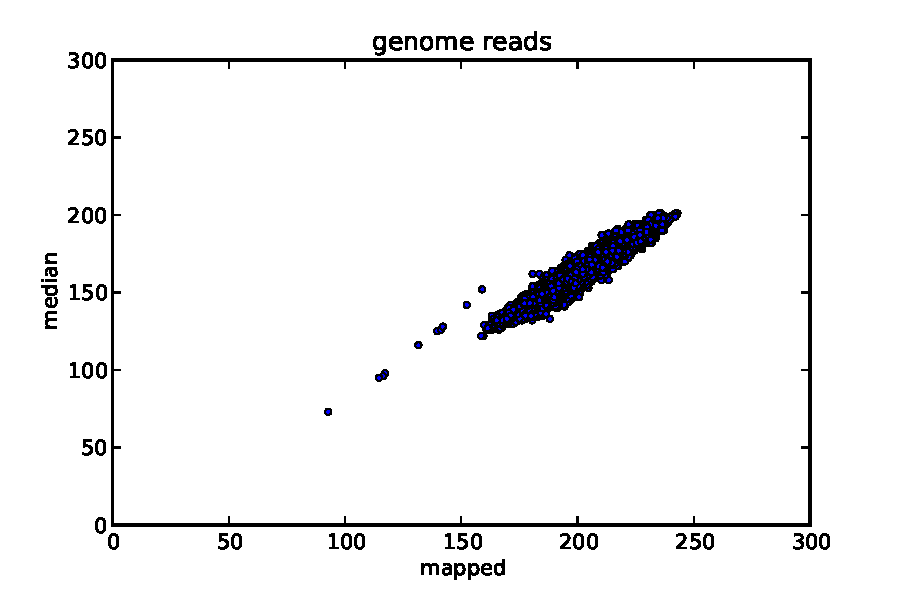
\includegraphics[width=4in]{diginorm-fig1a.pdf}
\end{center}
\caption{
{\bf Mapping and k-mer coverage measures correlate for uniform sampling on
both simulated data and real {\em E. coli} data.}
XXX
}
\label{fig:random}
\end{figure}

%@@CTB \section*{Figure Legends}

\begin{figure}[!ht]
\begin{center}
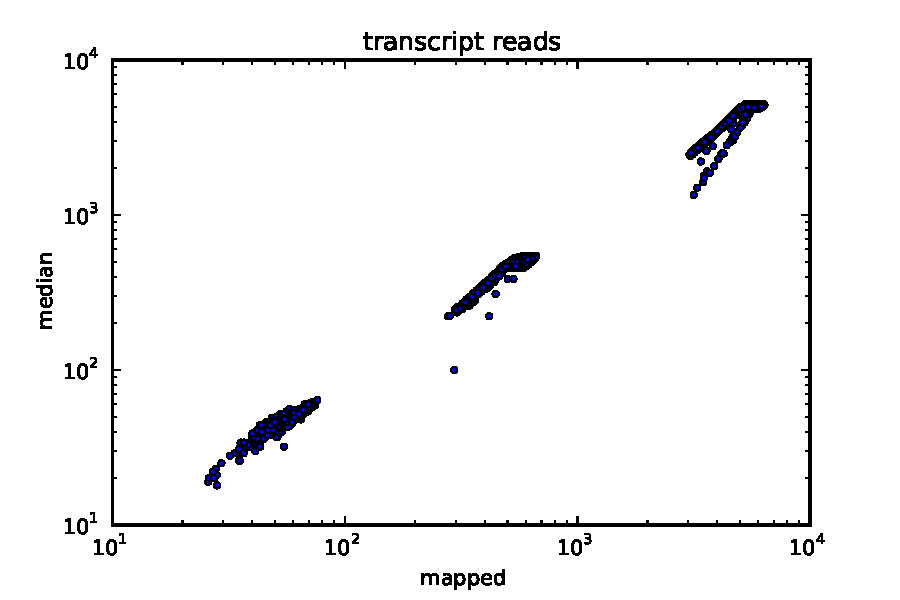
\includegraphics[width=4in]{diginorm-fig2a.pdf}
\end{center}
\caption{
{\bf Mapping and k-mer coverage measures correlate for biased samples.}
XXX
}
\label{fig:transcripts}
\end{figure}

\begin{figure}
\caption{
{\bf Coverage of simulated and real genomes, calculated from reads before and after normalization.}}
\label{fig:coverage}
\end{figure}

\begin{figure}
\caption{
{\bf Accumulation of reads.}}
\label{fig:accumulate}
\end{figure}

\begin{figure}
\caption{
{\bf Lost k-mers are always at end of real sequences.}}
\label{fig:supplEnd}
\end{figure}

\section*{Tables}

\begin{table}[!ht]
\caption{
\bf{Digital normalization to C=20 removes erroneous k-mers}}
\begin{tabular}{|l|c|c|c|c|}
Data set & True 20-mers & 20-mers in reads & 20-mers at C=20 & \% reads kept\\
\hline \\
Simulated genome & 399,981 & 8,162,813 & 3,052,007 (-2) & 19\% \\
Simulated mRNAseq & 48,100 & 2,466,638 (-88) & 1,087,916 (-9) & 4.1\% \\
{\em E. coli} genome & XXX & YYY & ZZZ & 11\% \\
Mouse mRNAseq & XXX & YYY & ZZZ & 28\% \\
\end{tabular}
\begin{flushleft} XXX
\end{flushleft}
\label{tab:normC20}
\end{table}

\begin{table}[!ht]
\caption{
\bf{Three-pass digital normalization removes most erroneous k-mers}}
\begin{tabular}{|l|c|c|c|c|}
Data set & True 20-mers & 20-mers in reads & 20-mers remaining & \% reads kept\\
\hline \\
Simulated genome & 399,981 & 8,162,813 & 453,588 (-4) & 5\% \\
Simulated mRNAseq & 48,100 & 2,466,638 (-88) & 182,855 (-351) & 1.2\% \\
{\em E. coli} genome & XXX & YYY & ZZZ & 2.1\% \\
Mouse mRNAseq & XXX & YYY & ZZZ & AA\% \\
\end{tabular}
\begin{flushleft} XXX
\end{flushleft}
\label{tab:normC5}
\end{table}

\end{document}

